\begin{figure}[t!]
    \centering

    \captionof{table}{请求间争用示例。}
    \label{tab:InterReqExample}

    \fontsize{9}{11}\selectfont
    \begin{tabular}{c|c|c|c|c}
        \toprule
        \textbf{请求 ID} & \textbf{流 ID} & \textbf{流大小} & \textbf{剩余时间} & \textbf{截止时间} \\
        \midrule
        1   & A & 2 & 9 & 18 \\
        2,3 & B & 4 & 6 & 12 \\
        4   & C & 3 & 0 & 7  \\
        \bottomrule
    \end{tabular}

    \begin{subfigure}{0.48\columnwidth}
        \centering
        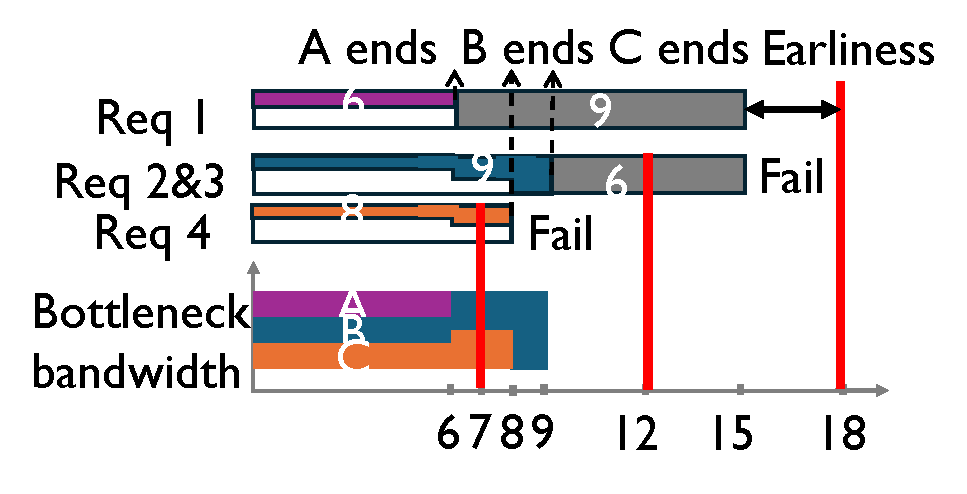
\includegraphics[width=\linewidth]{figures/methodology/InterContentionExample-FS.pdf}
        \caption{公平共享}
        \label{fig:bg:expfs}
    \end{subfigure}
    \hfill
    \begin{subfigure}{0.48\columnwidth}
        \centering
        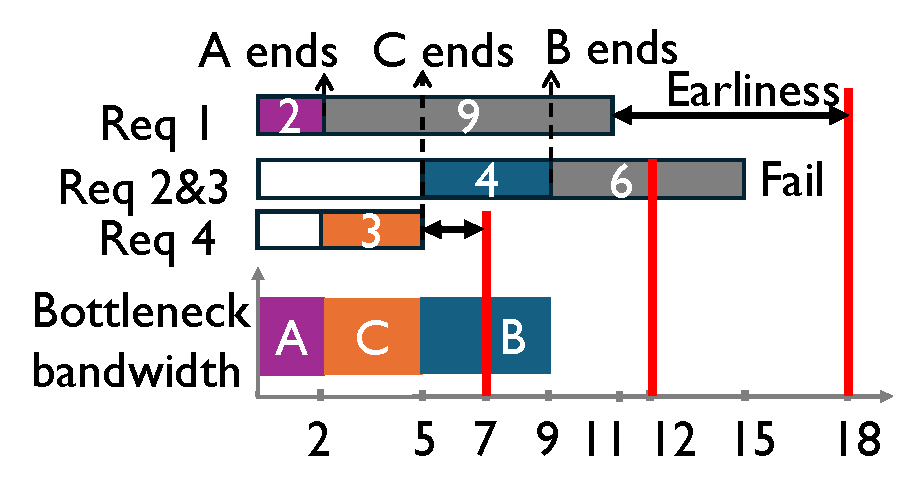
\includegraphics[width=\linewidth]{figures/methodology/InterContentionExample-SJF.pdf}
        \caption{最短作业优先}
        \label{fig:bg:expsjf}
    \end{subfigure}

    \par\medskip

    \begin{subfigure}{0.48\columnwidth}
        \centering
        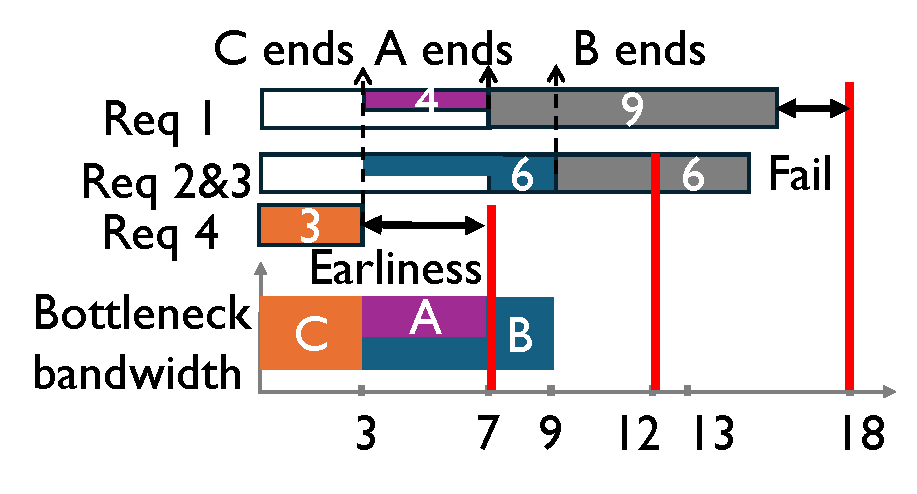
\includegraphics[width=\linewidth]{figures/methodology/InterContentionExample-EDF.pdf}
        \caption{最早截止时间优先}
        \label{fig:bg:expedf}
    \end{subfigure}
    \hfill
    \begin{subfigure}{0.48\columnwidth}
        \centering
        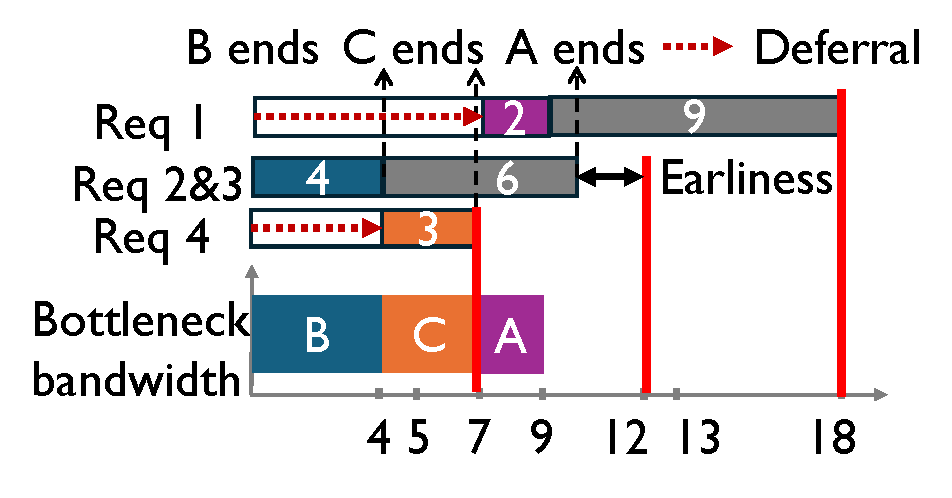
\includegraphics[width=\linewidth]{figures/methodology/InterContentionExample-DAP.pdf}
        \caption{延后并提升}
        \label{fig:bg:expopt}
    \end{subfigure}

    \caption{\textbf{请求间争用场景下不同调度策略的对比。}
    红色竖线表示硬截止时间，灰色条表示后续持续时间。
    (a) 公平共享和 (b) SJF 由于缺乏截止时间感知，无法保护紧急的 Flow-B；
    (c) EDF 会让具有显式但宽松截止时间的流不必要地过早完成；
    (d) \DAP 会有策略地延后非紧急流，以最小化提前量，
    并仅在必要时提升其优先级，从而实现\textit{恰好按时完成}。}
    \label{fig:meth:inter}

    \vspace{-2em}
\end{figure}
